\documentclass[12pt, letterpaper]{scrartcl}


\usepackage{fullpage} % Set margins and place page numbers at bottom center
\usepackage[shortlabels]{enumitem} % Use a. in the enumerate
\usepackage{amsmath} % aligned equations
\usepackage{graphicx} % include figure
\usepackage{float} % usage of H for figure float
\usepackage{amssymb} % \blacksqure
\usepackage{xhfill} % fill horizontal line

\usepackage{colortbl}
\usepackage{xcolor} % colors
\usepackage{sectsty} % section coloring
\usepackage{setspace}
\usepackage{bm}
\onehalfspacing
\sectionfont{\color{blue}}  % sets colour of sections

%%%%%%%%%%%%%%%%%%%%%%%%%%%%%%%%%%%%%%%%%%%%%%%%%%%%%%%%%%%%%%%%%%%%%%
% MY COMMANDS                                                        %
%%%%%%%%%%%%%%%%%%%%%%%%%%%%%%%%%%%%%%%%%%%%%%%%%%%%%%%%%%%%%%%%%%%%%%
\newcommand{\Z}{\mathbb{Z}}
\newcommand{\R}{\mathbb{R}}
\newcommand{\C}{\mathbb{C}}
\newcommand{\F}{\mathbb{F}}
\newcommand{\bigO}{\mathcal{O}}
\newcommand{\Real}{\mathcal{Re}}
\newcommand{\poly}{\mathcal{P}}
\newcommand{\mat}{\mathcal{M}}
\DeclareMathOperator{\Span}{span}
\newcommand{\Hom}{\mathcal{L}}
\DeclareMathOperator{\Null}{null}
\DeclareMathOperator{\Range}{range}
\newcommand{\defeq}{\vcentcolon=}
\newcommand{\restr}[1]{|_{#1}}
\newcommand*\diff{\mathop{}\!\mathrm{d}}


\begin{document}

% ### Header - start ###
\begin{center}
    \hrule
    \vspace{0.4cm}
    { \textbf{{\large Homework 3}} \\ MATH 564 --- Intermediate Differential Equations}
\end{center}
{ Name: \textbf{Ali Zafari} \hspace{\fill} Fall 2023 } \newline\hrule
% ### Header - end ###
% \section*{Exercises to be Considered \xrfill[2pt]{3pt}[blue]}
% \begin{itemize}[-]
%     \item 2.8.12
%     \item 2.8.17
%     \item 2.8.19
% \end{itemize}
% \vskip1mm\hrule

\section*{2.8 Autonomous Systems-Phase Space \xrfill[2pt]{3pt}[blue]}

\subsubsection*{Exercise 2.8.10}
\begin{itemize}
    \item eigenvalues:
    \begin{align*}
        \det 
        \left(\begin{array}{cc}
        -\lambda & v \\
        -v & -\lambda 
        \end{array}\right)=0
        \Longrightarrow
        \lambda_{1},\lambda_{2}=+iv, -iv
    \end{align*}
    \item eigenvectors:
    \begin{itemize}
        \item $\lambda_{1}=+iv$
        \begin{align*}
            \left(\begin{array}{cc}
            -iv & v \\
            -v & -iv 
            \end{array}\right)
            v_1=0
            \Longrightarrow
            v_1=\left(\begin{array}{c}
            c_1 \\
            ic_1 
            \end{array}\right)
        \end{align*}
        \item $\lambda_{1}=-iv$
        \begin{align*}
            \left(\begin{array}{cc}
            iv & v \\
            -v & iv 
            \end{array}\right)
            v_2=0
            \Longrightarrow
            v_2=\left(\begin{array}{c}
            c_2 \\
            -ic_2 
            \end{array}\right)
        \end{align*}
    \end{itemize}
    \item general solution (${\boldsymbol\eta}=\phi(0)$):
    \begin{align*}
        \phi(t)=
        e^{ivt}
        \left(\begin{array}{c}
            c_1 \\
            ic_1 
        \end{array}\right)
        +
        e^{-ivt}
        \left(\begin{array}{c}
            c_2 \\
            -ic_2 
        \end{array}\right)
        =
        \left(\begin{array}{c}
            \eta_1\cos vt +\eta_2 \sin vt\\
            -\eta_1\sin vt +\eta_2 \cos vt
        \end{array}\right)
    \end{align*}
    Using polar coordinates in which $y_1=r\cos\theta$ and $y_2=r\sin\theta$, by letting $\rho=\frac{1}{\sqrt{\eta_1^2+\eta_2^2}}$, $\cos \alpha=\frac{\eta_1}{\rho}$, $\sin \alpha=\frac{\eta_2}{\rho}$:

    \begin{align*}
        \phi(t)=\left(\begin{array}{c}
                \rho\cos(-(vt-\alpha))\\
                \rho\sin(-(vt-\alpha))
            \end{array}\right)
        \Longrightarrow
        r=\rho,\quad\theta=-(vt-\alpha)
    \end{align*}

    \item phase space ($v<0$):
    \begin{figure}[H]
    \centering
    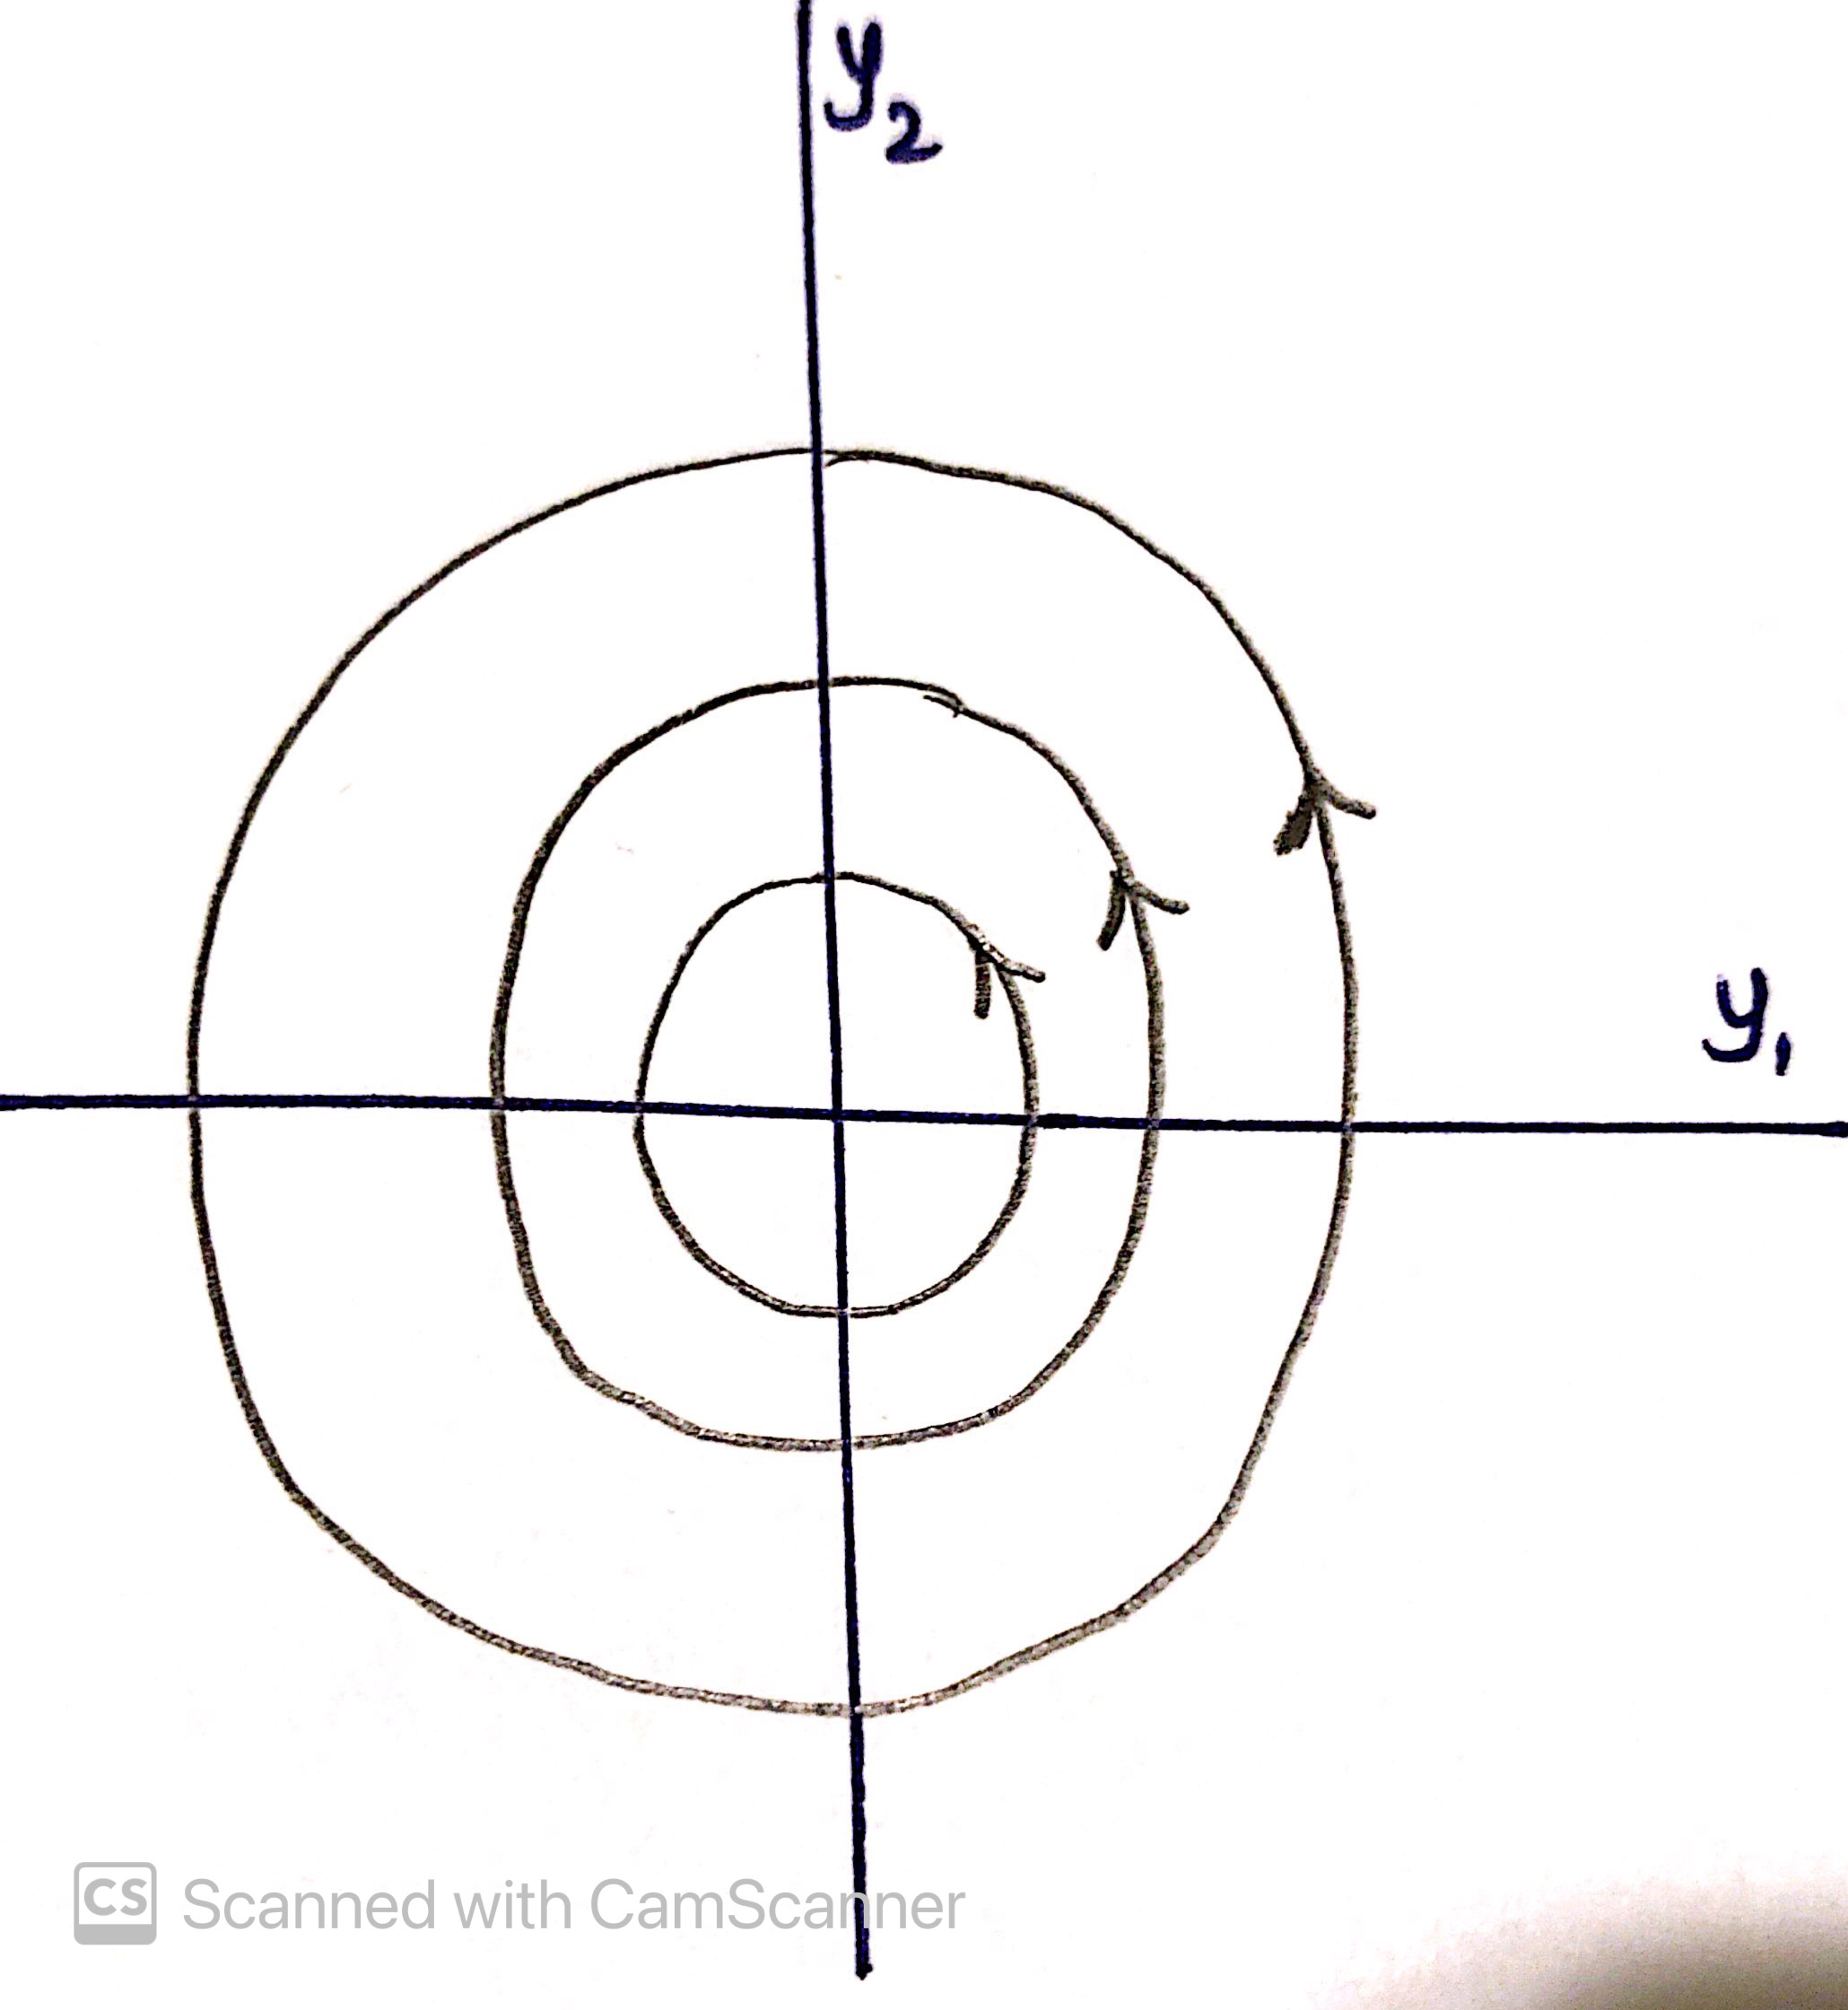
\includegraphics[width=0.3\textwidth]{fig/2.8.10.JPG}
    \end{figure}
\end{itemize}
\vskip1mm\hrule


\subsubsection*{Exercise 2.8.11}

\begin{itemize}
    \item change of variables, $y_1=x$ and $y_2=x'$:
    \begin{align*}
        \left(\begin{array}{c}
        y_1' \\
        y_2' 
        \end{array}\right)=
        \left(\begin{array}{cc}
        0 & 1 \\
        -1 & 0 
        \end{array}\right)
        \left(\begin{array}{c}
        y_1 \\
        y_2 
        \end{array}\right)
    \end{align*}
    \item eigenvalues:
    \begin{align*}
        \det 
        \left(\begin{array}{cc}
        -\lambda & 1 \\
        -1 & -\lambda 
        \end{array}\right)=0
        \Longrightarrow
        \lambda_{1},\lambda_{2}=+i, -i
    \end{align*}
    \item eigenvectors:
    \begin{itemize}
        \item $\lambda_{1}=+i$
        \begin{align*}
            \left(\begin{array}{cc}
            -i & 1 \\
            -1 & -i 
            \end{array}\right)
            v_1=0
            \Longrightarrow
            v_1=\left(\begin{array}{c}
            c_1 \\
            ic_1 
            \end{array}\right)
        \end{align*}
        \item $\lambda_{1}=-i$
        \begin{align*}
            \left(\begin{array}{cc}
            i & 1 \\
            -1 & i 
            \end{array}\right)
            v_2=0
            \Longrightarrow
            v_2=\left(\begin{array}{c}
            c_2 \\
            -ic_2 
            \end{array}\right)
        \end{align*}
    \end{itemize}
    \item general solution (${\boldsymbol\eta}=\phi(0)$):
    \begin{align*}
        \phi(t)=
        e^{it}
        \left(\begin{array}{c}
            c_1 \\
            ic_1 
        \end{array}\right)
        +
        e^{-it}
        \left(\begin{array}{c}
            c_2 \\
            -ic_2 
        \end{array}\right)
        =
        \left(\begin{array}{c}
            \eta_1\cos t +\eta_2 \sin t\\
            -\eta_1\sin t +\eta_2 \cos t
        \end{array}\right)
    \end{align*}
    Using polar coordinates in which $y_1=r\cos\theta$ and $y_2=r\sin\theta$, by letting $\rho=\frac{1}{\sqrt{\eta_1^2+\eta_2^2}}$, $\cos \alpha=\frac{\eta_1}{\rho}$, $\sin \alpha=\frac{\eta_2}{\rho}$:

    \begin{align*}
        \phi(t)=\left(\begin{array}{c}
                \rho\cos(-(t-\alpha))\\
                \rho\sin(-(t-\alpha))
            \end{array}\right)
        \Longrightarrow
        r=\rho,\quad\theta=-(t-\alpha)
    \end{align*}

    \item phase space (origin is not an attractor point):
    \begin{figure}[H]
    \centering
    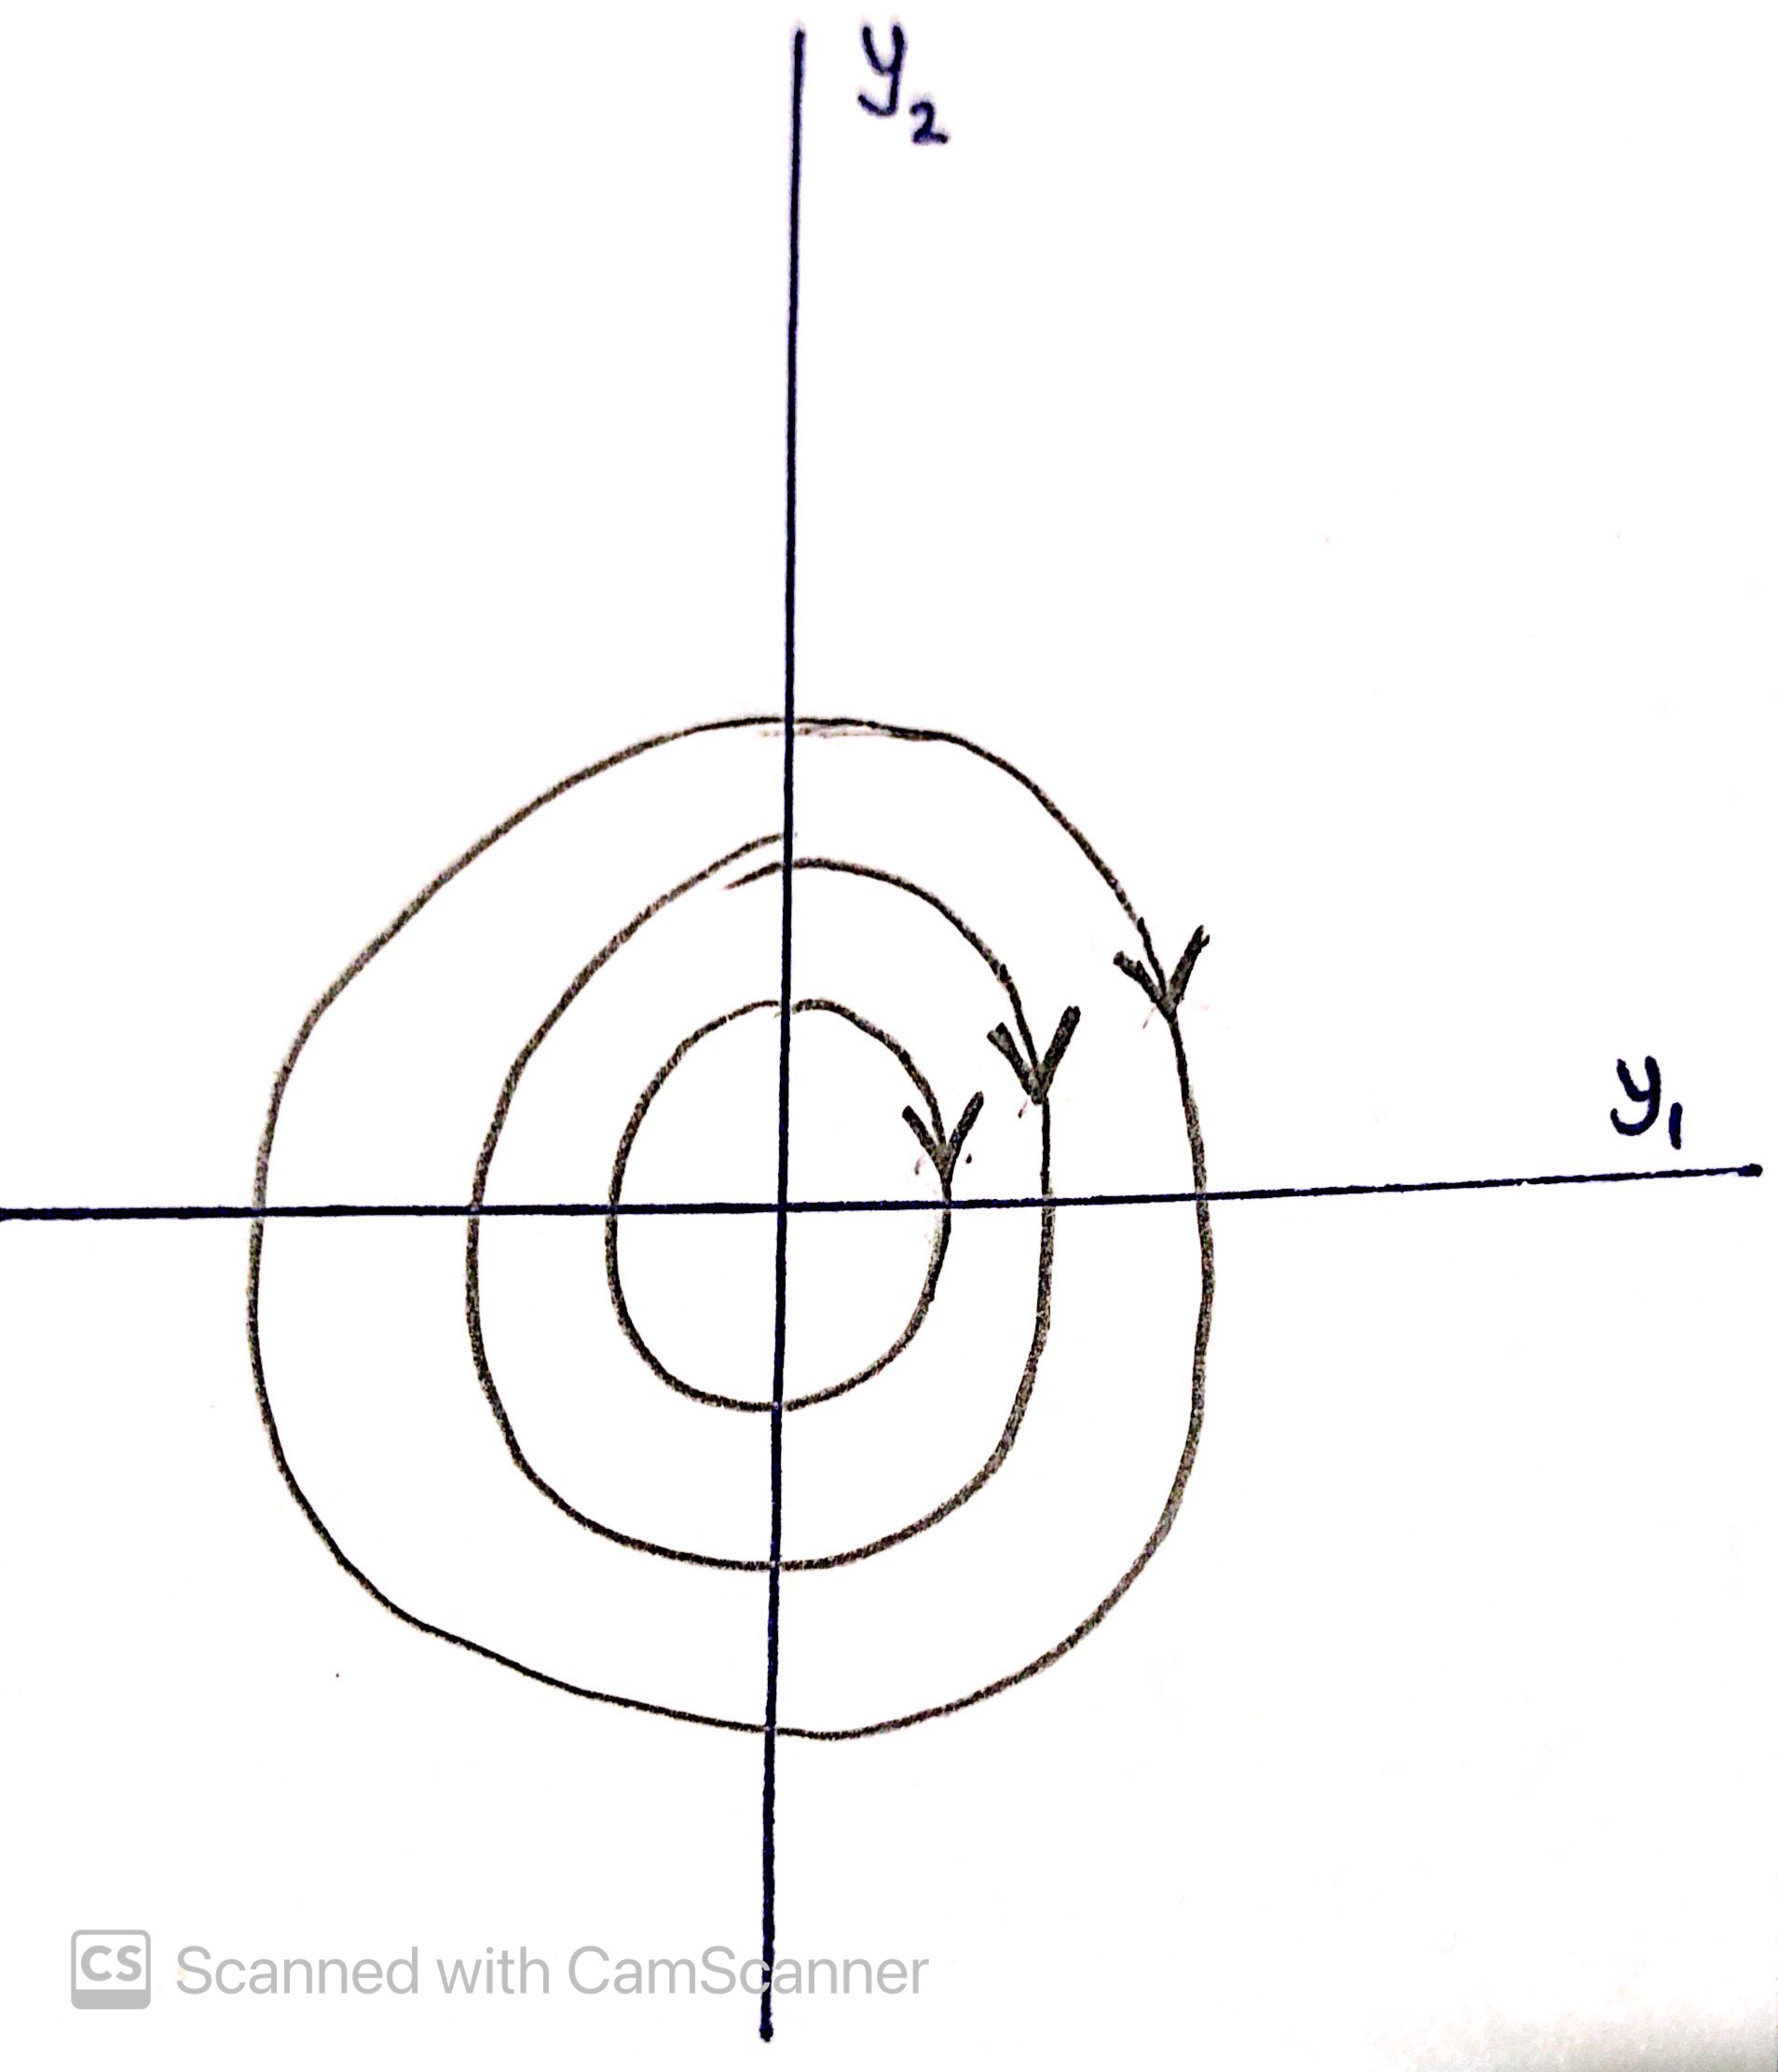
\includegraphics[width=0.3\textwidth]{fig/2.8.11.JPG}
    \end{figure}
\end{itemize}
\vskip1mm\hrule


\subsubsection*{Exercise 2.8.12}
\begin{itemize}
    \item change of variables, $y_1=x$ and $y_2=x'$:
    \begin{align*}
        \left(\begin{array}{c}
        y_1' \\
        y_2' 
        \end{array}\right)=
        \left(\begin{array}{cc}
        0 & 1 \\
        -1 & 3 
        \end{array}\right)
        \left(\begin{array}{c}
        y_1 \\
        y_2 
        \end{array}\right)
    \end{align*}
    \item eigenvalues:
    \begin{align*}
        \det 
        \left(\begin{array}{cc}
        -\lambda & 1 \\
        -1 & 3-\lambda 
        \end{array}\right)=0
        \Longrightarrow
        \lambda_{1},\lambda_{2}=\frac{3+\sqrt{5}}{2}, \frac{3-\sqrt{5}}{2}
    \end{align*}
    \item eigenvectors:
    \begin{itemize}
        \item $\lambda_{1}=\frac{3+\sqrt{5}}{2}$
        \begin{align*}
            \left(\begin{array}{cc}
            -\frac{3+\sqrt{5}}{2} & 1 \\
            -1 & \frac{3-\sqrt{5}}{2} 
            \end{array}\right)
            v_1=0
            \Longrightarrow
            v_1=\left(\begin{array}{c}
            \frac{3-\sqrt{5}}{2}c_1 \\
             c_1
            \end{array}\right)
        \end{align*}
        \item $\lambda_{1}=\frac{3-\sqrt{5}}{2}$
        \begin{align*}
            \left(\begin{array}{cc}
            -\frac{3-\sqrt{5}}{2} & 1 \\
            -1 & \frac{3+\sqrt{5}}{2} 
            \end{array}\right)
            v_2=0
            \Longrightarrow
            v_2=\left(\begin{array}{c}
            \frac{3+\sqrt{5}}{2} c_2 \\
            c_2
            \end{array}\right)
        \end{align*}
    \end{itemize}
    \item general solution (${\boldsymbol\eta}=\phi(0)$):
    \begin{align*}
        \phi(t)=
        e^{\frac{3+\sqrt{5}}{2}t}
        \left(\begin{array}{c}
            \frac{3-\sqrt{5}}{2}c_1 \\
             c_1 
        \end{array}\right)
        +
        e^{\frac{3-\sqrt{5}}{2}t}
        \left(\begin{array}{c}
            \frac{3+\sqrt{5}}{2} c_2 \\
            c_2
        \end{array}\right)
    \end{align*}
    where $\frac{3-\sqrt{5}}{2}c_1+\frac{3+\sqrt{5}}{2} c_2=\eta_1$ and $c_1+c_2=\eta_2$.
    
    \item phase space (origin is not an attractor point):
    
    \begin{figure}[H]
    \centering
    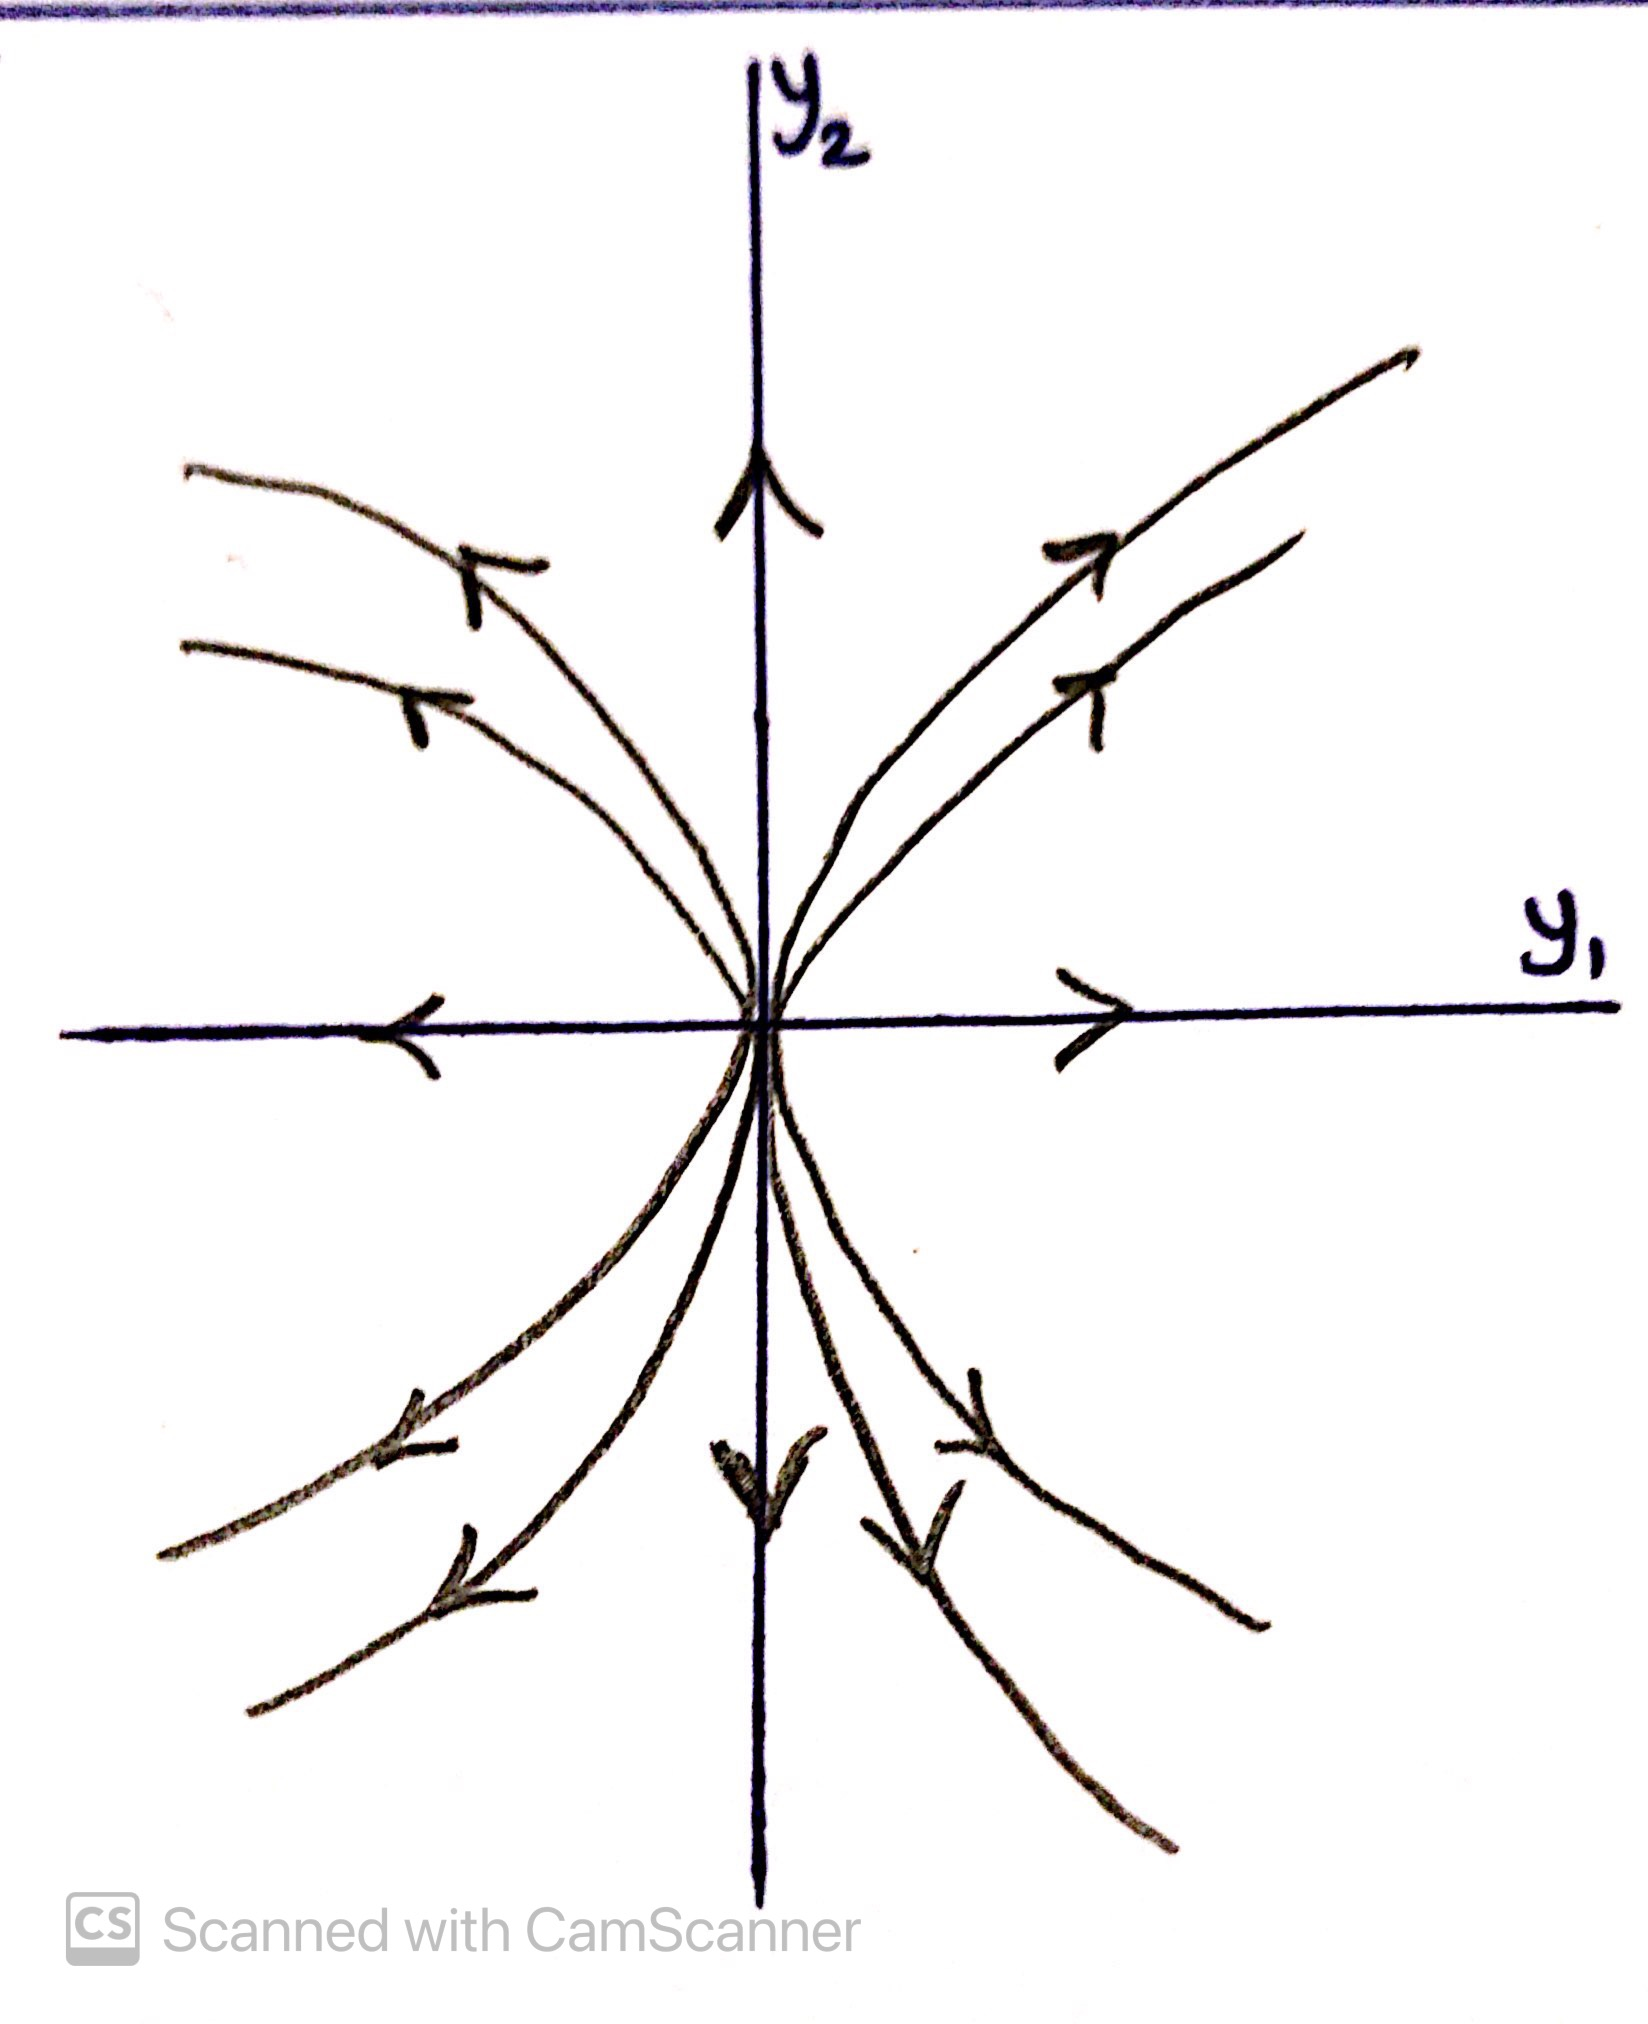
\includegraphics[width=0.3\textwidth]{fig/2.8.12.JPG}
    \end{figure}
\end{itemize}
\vskip1mm\hrule

\subsubsection*{Exercise 2.8.17}
\begin{itemize}
    \item change of variables, $y_1=x$ and $y_2=x'$:
    \begin{align*}
        \left(\begin{array}{c}
        y_1' \\
        y_2' 
        \end{array}\right)=
        \left(\begin{array}{cc}
        0 & 1 \\
        -1 & 2 
        \end{array}\right)
        \left(\begin{array}{c}
        y_1 \\
        y_2 
        \end{array}\right)
    \end{align*}
    \item eigenvalues:
    \begin{align*}
        \det 
        \left(\begin{array}{cc}
        -\lambda & 1 \\
        -1 & 2-\lambda 
        \end{array}\right)=0
        \Longrightarrow
        \lambda_{1},\lambda_{2}=1, 1
    \end{align*}
    \item eigenvectors:
        Any vector in $\mathbb{F}^2$ can be assumed as generalized eigenvector.
    \item general solution (${\boldsymbol\eta}=\phi(0)$):
    \begin{align*}
        \phi(t)=
        e^{t}
        \left[
        \left(\begin{array}{cc}
        1 & 0 \\
        0 & 1 
        \end{array}\right)
        +
        \left(\begin{array}{cc}
        -t & t \\
        -t & t 
        \end{array}\right)
        \right]
        \left(\begin{array}{c}
            \eta_1\\
            \eta_2
        \end{array}\right)
        =
        e^t
        \left(\begin{array}{c}
            (\eta_2-\eta_1)t+\eta_1\\
            (\eta_2-\eta_1)t+\eta_2
        \end{array}\right)
    \end{align*}

    \item phase space (origin is an attractor point):
    \begin{figure}[H]
    \centering
    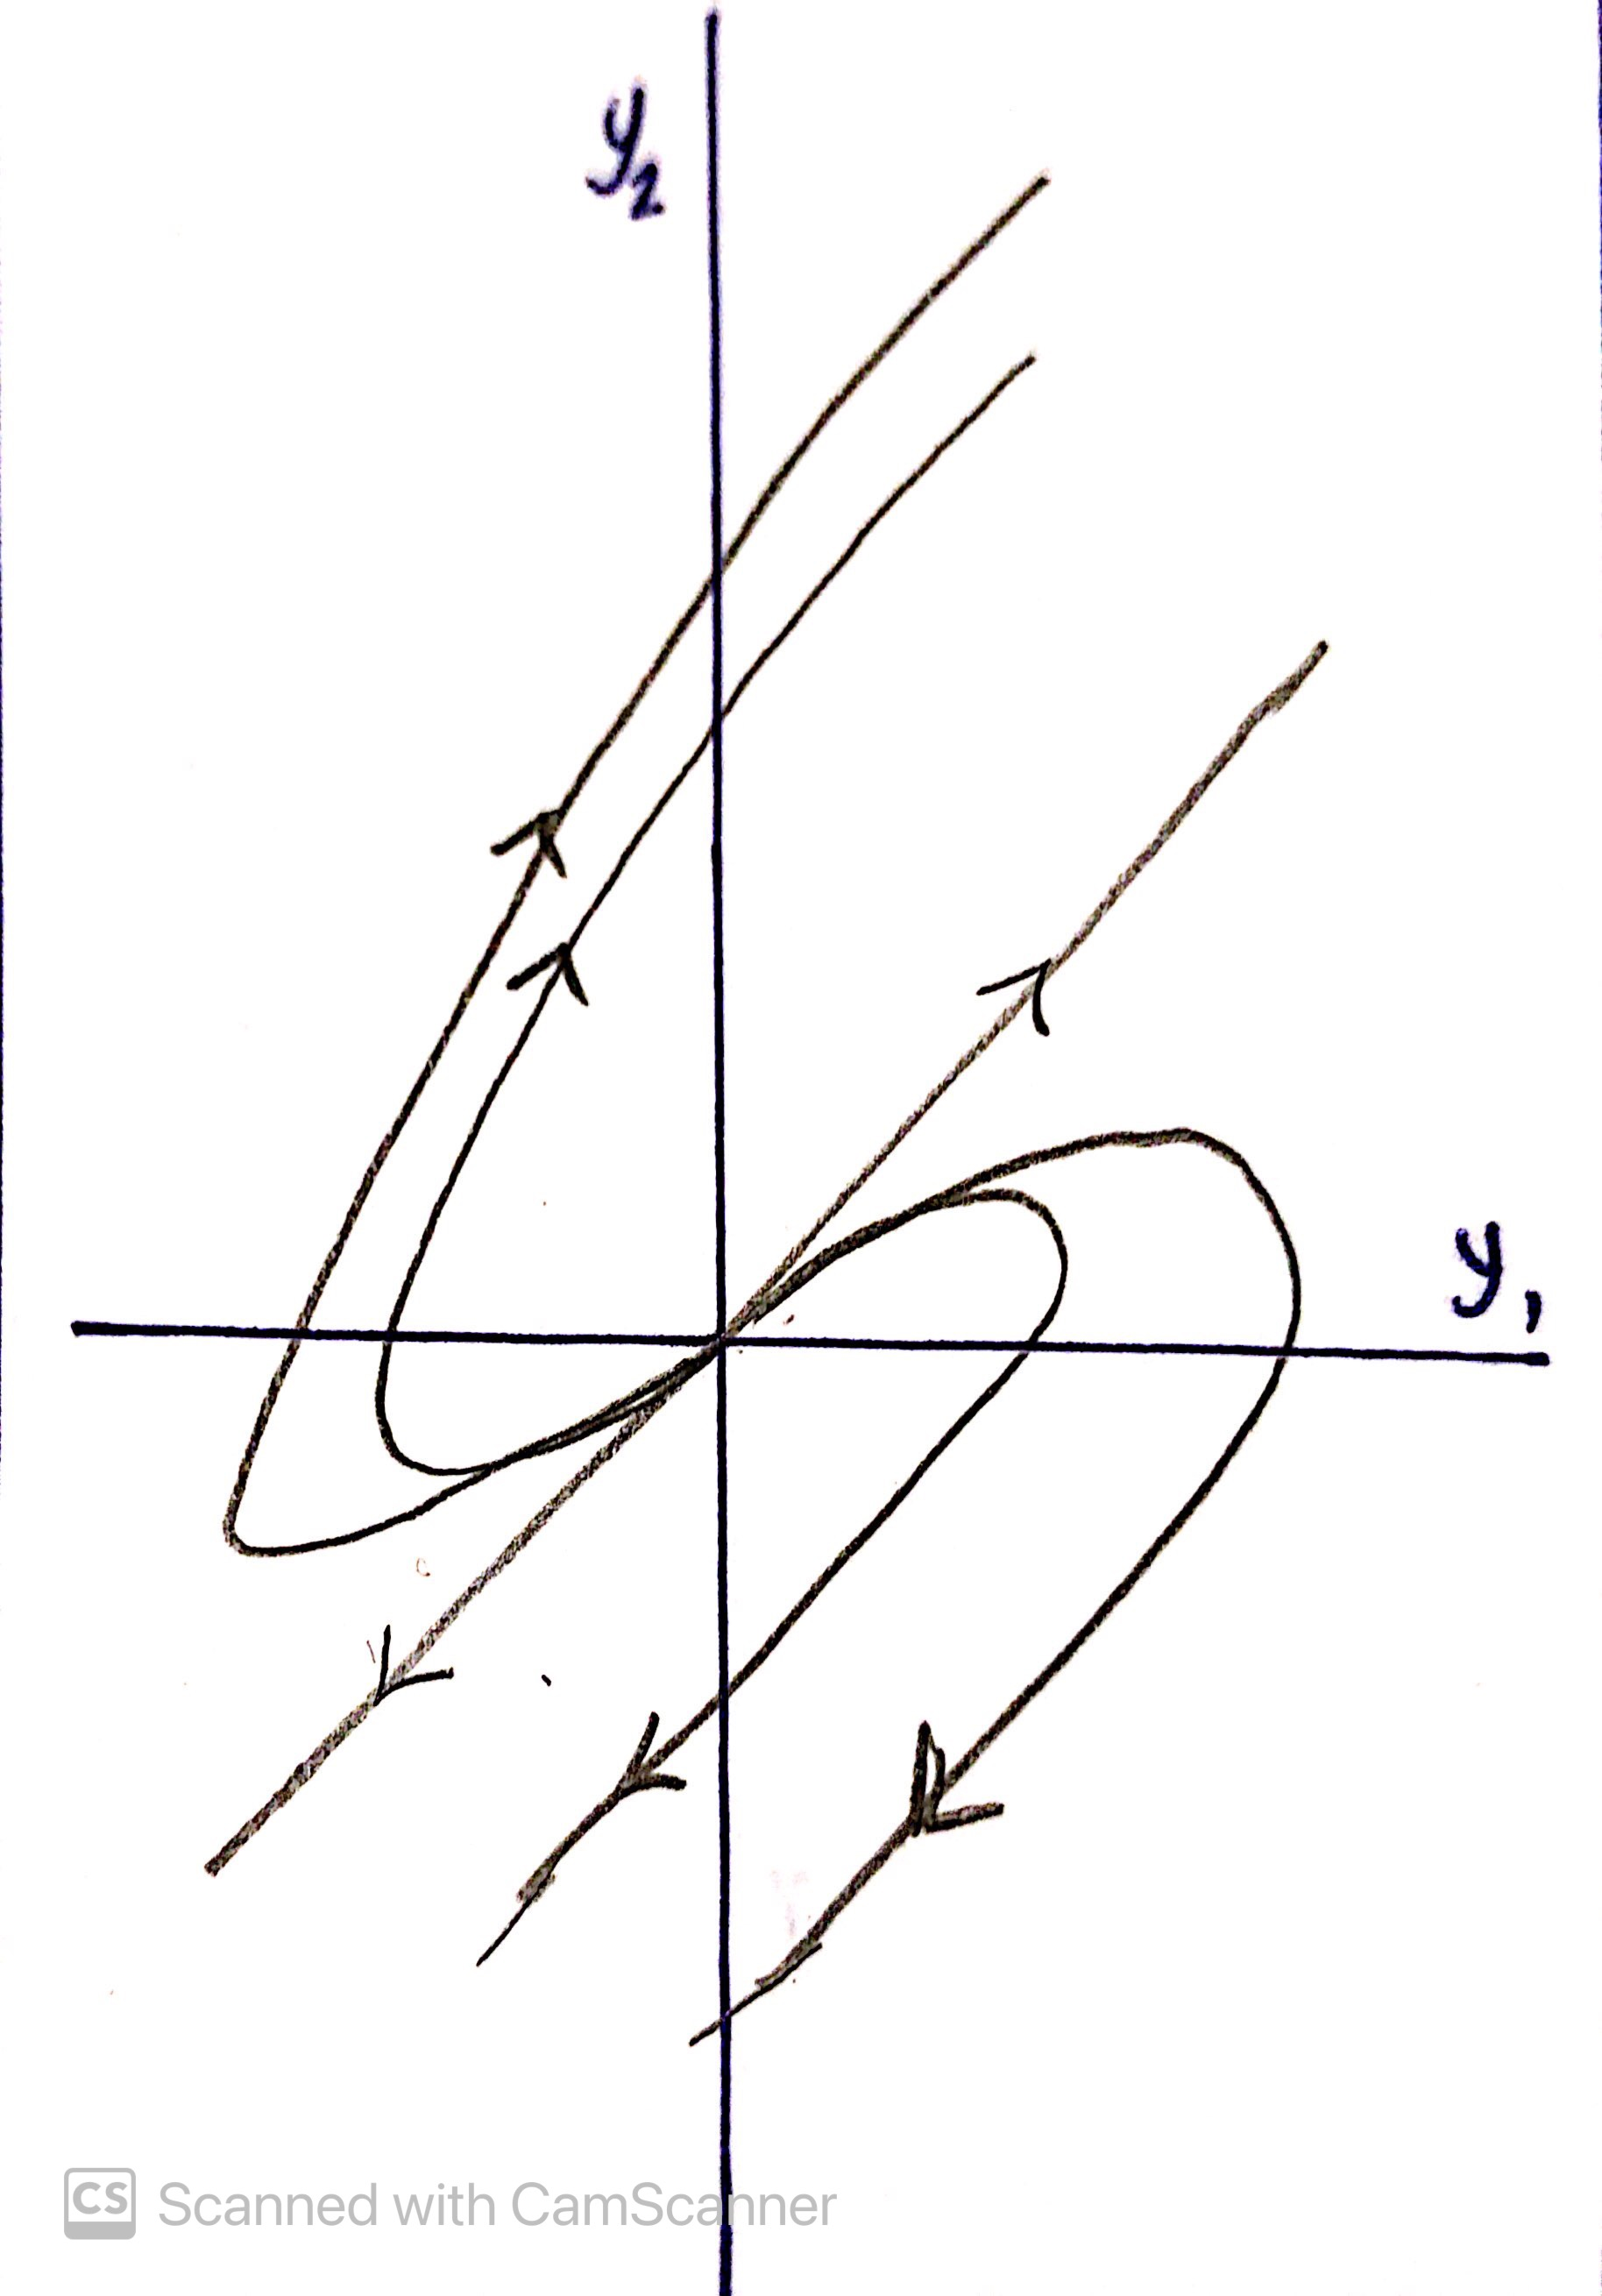
\includegraphics[width=0.3\textwidth]{fig/2.8.17.JPG}
    \end{figure}
\end{itemize}
\vskip1mm\hrule


\subsubsection*{Exercise 2.8.19}
\begin{enumerate}[(a)]
    \item 
    \begin{itemize}
    \item system of differential equations:
    \begin{align*}
        \left(\begin{array}{c}
        y_1' \\
        y_2' 
        \end{array}\right)=
        \left(\begin{array}{cc}
        1 & -1 \\
        2 & -2 
        \end{array}\right)
        \left(\begin{array}{c}
        y_1 \\
        y_2 
        \end{array}\right)
    \end{align*}
    \item eigenvalues:
    \begin{align*}
        \det 
        \left(\begin{array}{cc}
        1-\lambda & -1 \\
        2 & -2-\lambda 
        \end{array}\right)=0
        \Longrightarrow
        \lambda_{1},\lambda_{2}=0, -1
    \end{align*}
    \item eigenvectors:
        \begin{itemize}
        \item $\lambda_{1}=0$
        \begin{align*}
            \left(\begin{array}{cc}
            1 & -1 \\
            2 & -2 
            \end{array}\right)
            v_1=0
            \Longrightarrow
            v_1=\left(\begin{array}{c}
            c_1 \\
            c_1 
            \end{array}\right)
        \end{align*}
        \item $\lambda_{1}=-1$
        \begin{align*}
            \left(\begin{array}{cc}
            2 & -1 \\
            2 & -1 
            \end{array}\right)
            v_2=0
            \Longrightarrow
            v_2=\left(\begin{array}{c}
            c_2 \\
            2c_2 
            \end{array}\right)
        \end{align*}
    \end{itemize}
    \item general solution (${\boldsymbol\eta}=\phi(0)$):
    \begin{align*}
        \phi(t)=
        \left(\begin{array}{c}
            c_1 \\
            c_1 
        \end{array}\right)
        +
        e^{-t}
        \left(\begin{array}{c}
            c_2 \\
            2c_2 
        \end{array}\right)
        =
        \left(\begin{array}{c}
            2\eta_1-\eta_2+e^{-t}(\eta_2-\eta_1) \\
            2\eta_1-\eta_2+2e^{-t}(\eta_2-\eta_1) 
        \end{array}\right)
    \end{align*}
    \end{itemize}

    All points on the line $y_1=y_2$ are critical points.
    \item phase space: 
    \begin{figure}[H]
    \centering
    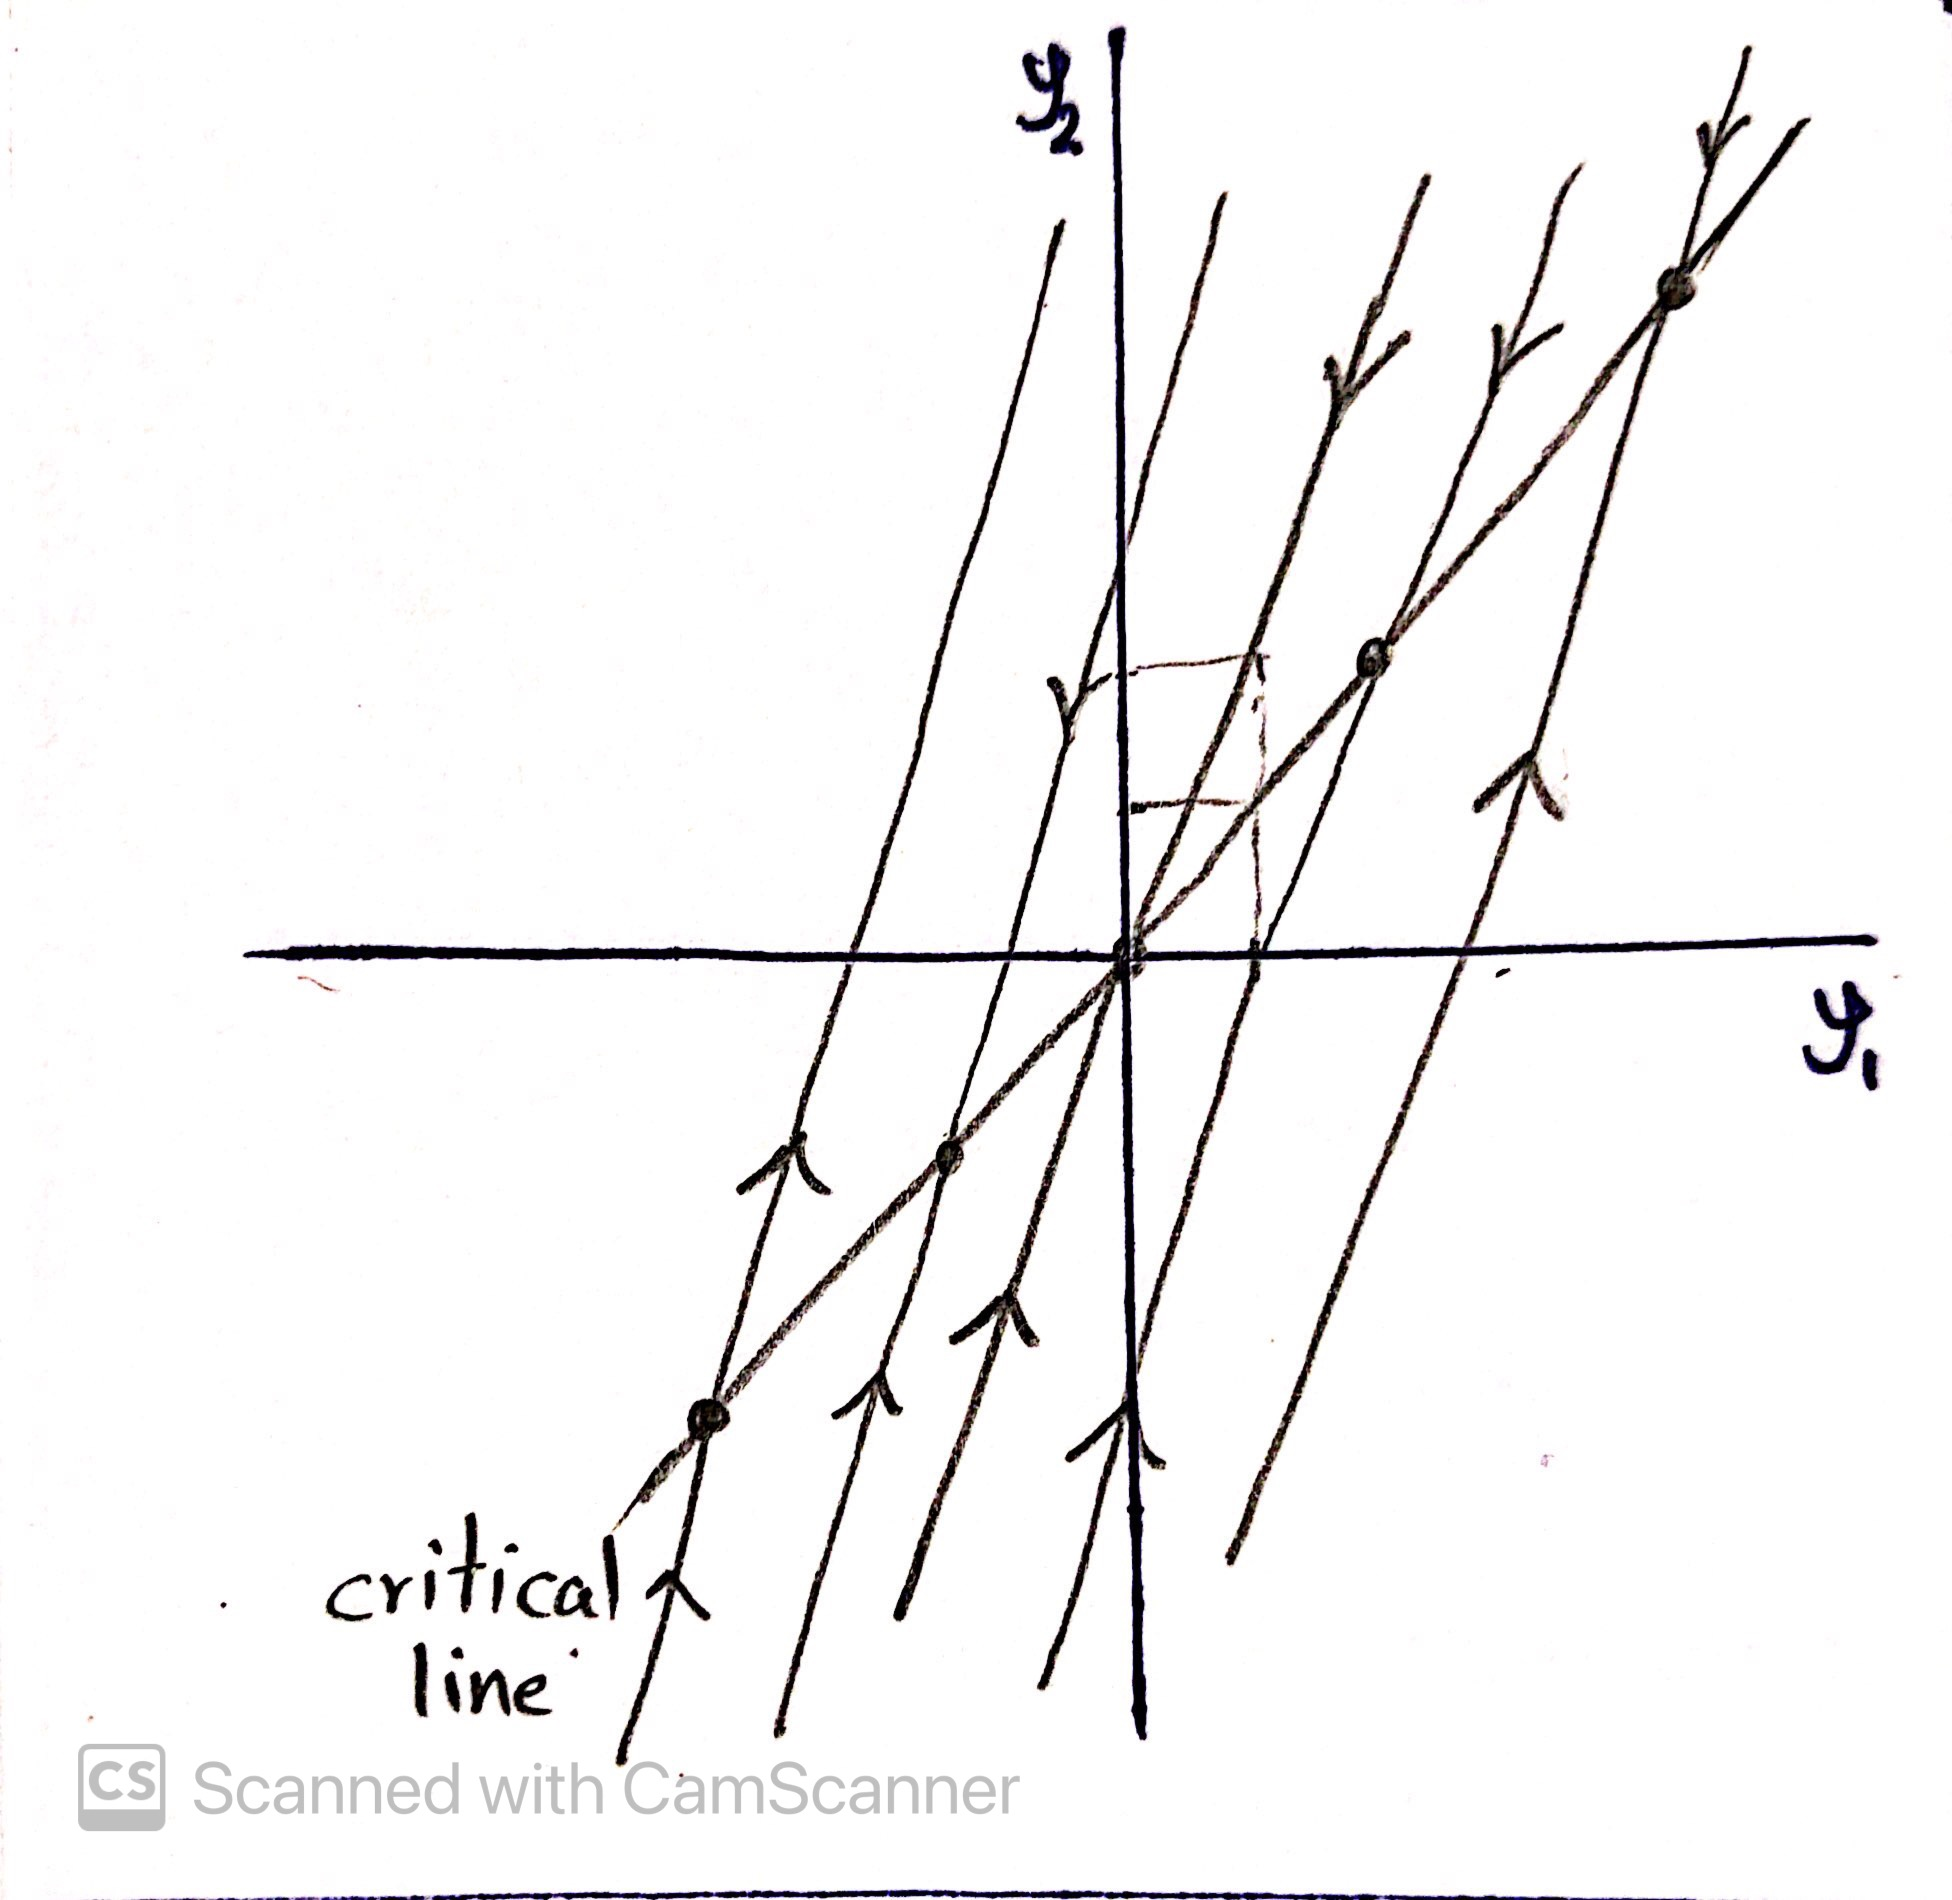
\includegraphics[width=0.3\textwidth]{fig/2.8.19.JPG}
    \end{figure}
\end{enumerate}
\vskip1mm\hrule


\end{document}